\documentclass[10pt,a4paper,spanish]{article}

\usepackage[spanish]{babel}
\usepackage[utf8]{inputenc}
\usepackage{amsmath, amsthm}
\usepackage{amsfonts, amssymb, latexsym}
\usepackage{enumerate}
% \usepackage[official]{eurosym}
\usepackage{graphicx}
\usepackage[usenames, dvipsnames]{color}
\usepackage{colortbl}
\usepackage{multirow}
\usepackage{fancyhdr}
\usepackage[all]{xy}
% \usepackage{minted}
\usepackage{float}
\usepackage{subfigure}
\usepackage{tikz}
\usepackage{pgfplots}
\usepackage{cancel}
\pgfplotsset{compat=1.5}

\usepackage[top=2.5cm, bottom=2.5cm, left=3cm, right=3cm]{geometry}

\usepackage[bookmarks=true,
            bookmarksnumbered=false, % true means bookmarks in
                                     % left window are numbered
            bookmarksopen=false,     % true means only level 1
                                     % are displayed.
            colorlinks=true,
            linkcolor=red,
            citecolor=blue]{hyperref}

\newcommand{\HRule}{\rule{\linewidth}{0.5mm}} % regla horizontal para  el titulo

\pagestyle{plain}
%con esto nos aseguramos de que las cabeceras de capítulo y de sección vayan en minúsculas

\fancyhf{} %borra cabecera y pie actuales
% \fancyhead[LE,RO]{}
% \fancyhead[LO]{}
\fancyfoot[C]{\thepage}
% \renewcommand{\headrulewidth}{0.5pt}
% \renewcommand{\footrulewidth}{0pt}
% \addtolength{\headheight}{0.5pt} %espacio para la raya
% \fancypagestyle{plain}{%
%       \fancyhead{} %elimina cabeceras en páginas "plain"
%       \renewcommand{\headrulewidth}{0pt} %así como la raya
% }

% %%%%% Para cambiar el tipo de letra en el título de la sección %%%%%%%%%%%
% \usepackage{sectsty}
% \chapterfont{\fontfamily{frc}\selectfont}
% \sectionfont{\fontfamily{pag}\selectfont}
% \subsectionfont{\fontfamily{pag}\selectfont}
% \subsubsectionfont{\fontfamily{pag}\selectfont}

% \newmintedfile[mycplusplus]{c++}{
%     linenos,
%     numbersep=5pt,
%     gobble=0,
%     frame=lines,
%     framesep=2mm,
%     tabsize=3,
% }

% \newmintedfile[mypython]{python}{
%     linenos,
%     numbersep=5pt,
%     gobble=0,
%     frame=lines,
%     framesep=2mm,
%     tabsize=3,
% }

\definecolor{amaranth}{rgb}{0.9, 0.17, 0.31}

\usepackage{arev}
\usepackage[T1]{fontenc}

\setlength{\parindent}{0pt}
\setlength{\parskip}{1ex plus 0.5ex minus 0.2ex}

% \usepackage{titlesec}

% % \titleformat{\chapter}{\normalfont\huge\center}{--- \thechapter ---}{20pt}{}

% \titleformat
% {\chapter} % command
% [display] % shape
% {\Huge\center\bfseries} % format
% {--- \thechapter ---} % label
% {0.5ex} % sep
% {
%     \rule{\textwidth}{1pt}
%     \vspace{1ex}
%     \centering
% } % before-code
% [
% \vspace{-0.5ex}%
% \rule{\textwidth}{0.3pt}
% ] % after-code

%Definimos autor y título
\title{\Huge Arquitectura de las Redes \textit{Tor}}
\author{\Large Marta Gómez Macías y Braulio Vargas López}

\begin{document}
\renewcommand{\tablename}{Tabla}
\maketitle

\section{¿Qué es \textit{Tor}?}
Según \cite{deftor}, ``la red Tor es un grupo de servidores operativos voluntarios que permiten a las personas mejorar su privacidad y seguridad en Internet''. Esto quiere decir que una conexión a través de Tor nunca será directa, sino que pasará por estos servidores voluntarios para que no se pueda saber quién manda el paquete ni a dónde va dirigido. Además, Tor también se define como ``una efectiva herramienta para la elusión de la censura, permitiendo a sus usuarios acceder a contenido que de otra forma se encontraría bloqueado.''

\subsection{¿Por qué es \textit{Tor} más seguro que otras herramientas?}
Tal y como se explica en \cite{deftor}, usando Tor nos protegemos contra el ``análisis de tráfico''. Aunque el \textit{payload} de los paquetes que enviamos a través de la red se encuentre encriptado, la cabecera normalmente no suele estarlo ya que se necesita para dirigir el paquete. Ésta cabecera facilita a los ``sniffers'' muchísima información sobre lo que estamos haciendo ya que incluye información como el ``host'' emisor, el ``host'' destino, el tamaño, el puerto al que va dirigido, etc.

¿La solución? Usar una red distribuida y anónima.

\section{¿Cómo mantiene \textit{Tor} el anonimato?}

El anonimato en \textit{Tor} se mantiene distribuyendo los paquetes que enviamos y recibimos por una gran cantidad de puntos distribuidos por internet, antes de llegar al destino, en vez de hacer una conexión directa entre el origen y el destino. Los paquetes de datos seguirán un camino aleatorio entre los distintos ``relevos'' que existen en la red de Tor, que eliminan nuestras $huellas$, para que en ningún punto del camino que toma el paquete se pueda saber de dónde viene el paquete y a dónde va.

Para crear un camino en la red privada de Tor, se crea un circuito incremental de conexiones encriptadas a través de los ``relevos'' de la red, como podemos ver en la \hyperref[htw1]{Figura \ref*{htw1}}. Los incrementos del circuito se hacen de uno en uno cada vez, y cada punto del circuito sólo sabe de qué relevo viene el paquete, y a qué relevo se lo tiene que dar. El cliente aporta un conjunto de llaves diferentes para encriptar el mensaje para cada punto del circuito para asegurarse de que en cada punto del circuito no se pueda seguir el paquete (\hyperref[htw2]{Figura \ref*{htw2}}). Gracias a esto, como un nodo solo conoce de qué nodo viene la información y a qué nodo tiene que mandarla, 

Por eficiencia, el mismo circuito tiene una vida de 10 minutos más o menos. Para las siguientes conexiones obtienen un nuevo circuito, como se ve en la \hyperref[htw3]{Figura \ref*{htw3}}.

\begin{figure}[H]
    \centering
    
    \mbox {
        \subfigure[Inicio de la conexión Tor. Al inicio de la conexión obtenemos una lista de nodos Tor del directorio del servidor.]{
            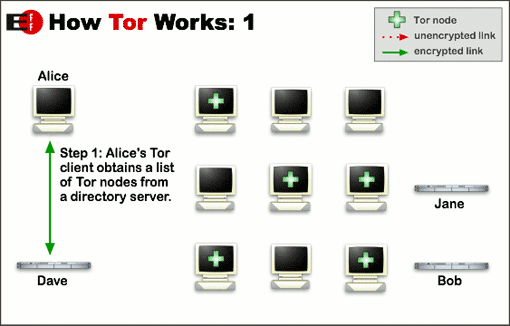
\includegraphics[width=0.5\textwidth]{htw1}
            \label{htw1}
        }
        
        \qquad
    
        \subfigure[Circuito o camino creado para la conexión. Como se ve en la imagen, los enlaces en verde están encriptados y los rojos no.] {
            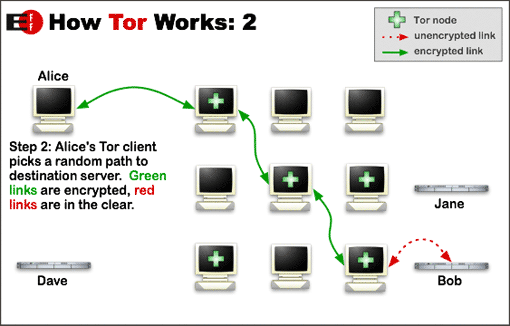
\includegraphics[width=0.51\textwidth]{htw2}
            \label{htw2}
        }
    }

    \mbox{
        \subfigure[Si se realiza una conexión más allá de esos 10 minutos, se genera un nuevo circuito.] {
            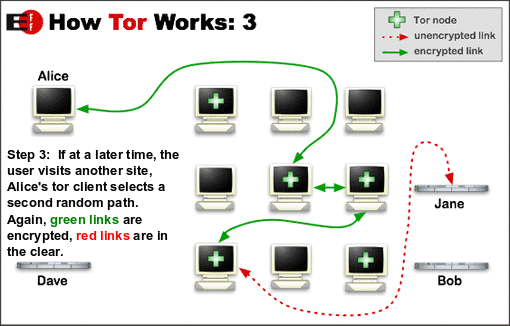
\includegraphics[width=0.51\textwidth]{htw3}
            \label{htw3}
        }
    }
    \caption{Cómo funciona Tor.}
    \label{htw}
\end{figure} 

\section{Arquitectura}

Tor solo funciona con flujos TCP y puede ser usado con cualquier aplicación with SOCKS support % Traducir al español plis

\section{Protocolo}

El protocolo de Tor se basa en una serie de protocolos seguros y parámetros de seguridad para la comunicación y envío de información. Es decir, es un protocolo \textit{End-to-End encryption}, en el que los datos se encriptan para poder enviarlos a través de un canal vulnerable, hasta que llegan al destinatario, donde puede ser desencriptado.

Para ello utiliza lo siguiente:

\begin{description}
    \item [Cifrado de \textit{stream}:] En este caso, cifra el \textit{stream} de datos mediante el algoritmo $AES-128~bits$
    \item [Cifrado de llave pública:] Para ello, utiliza claves $RSA$ con 1024-$bits$ (y un exponente fijo de 65537).
    \item [Protocolo Diffie-Hellman:] consiste en un protocolo criptográfico para establecer claves entre dos partes que no han tenido contacto previo, a través de un canal inseguro y anónimamente. Este protocolo consiste en coger un número primo al azar conococido, es decir público, y un número perteneciente al anillo formado por el primo inferior que será privado. Entonces, ambas partes hacen operaciones matemáticas con estos números que incluyen la exponenciación y se pasan los resultados. Ambas partes, con los números que disponen son capaces de llegar a la misma solución o clave.
    \item [Función Hash:] se usa para hacer el digest de los datos. Para ello utiliza el algoritmo SHA-1.
\end{description}

El tráfico que fluye a través del circuito, se envía en celdas de tamaño fijo, envueltas por una clave simétrica en cada nodo y enviada al siguiente nodo del circuito. 

\section{Ejemplo con Wireshark}

\bibliography{resumen.bib} %archivo citas.bib que contiene las entradas 
\bibliographystyle{siam} % haycle varias formas de citar

\end{document}